\documentclass[11pt,twoside]{amsart}
\usepackage{amssymb, amsmath, enumerate, libertine, microtype, hyperref,tikz-cd,hyperref}
\usepackage[normalem]{ulem}
\usepackage{fullpage}
\usepackage[T1]{fontenc}
\renewcommand{\labelitemi}{$\cdot$}
\usepackage{mathrsfs}
\usepackage{phaistos}
\definecolor{dark-red}{rgb}{0.4,0.15,0.15}
%   \definecolor{dark-blue}{rgb}{0.15,0.15,0.4}
%   \definecolor{medium-blue}{rgb}{0,0,0.5}
\setcounter{secnumdepth}{2}
\setcounter{tocdepth}{1}
\hypersetup{
    colorlinks, linkcolor=dark-red,
    citecolor=dark-red, urlcolor=dark-red
}


\theoremstyle{plain}
\newtheorem{prop}{Proposition}%[section]
\newtheorem{lemma}[prop]{Lemma}
\newtheorem{thm}[prop]{Theorem}
\newtheorem{obs}[prop]{Observation}
\newtheorem{app}[prop]{Application}
\newtheorem*{MainThm}{Main Theorem}
\newtheorem{cor}[prop]{Corollary}
\newtheorem{conj}[prop]{Conjecture}
\theoremstyle{remark}
\newtheorem{rmk}[prop]{Remark}
\newtheorem{prob}{Problem}
\newtheorem{bonus}[prop]{Bonus Problem}
\newtheorem{exc}{Exercise}
\theoremstyle{definition}
\newtheorem{ex}[prop]{Example}
\theoremstyle{definition}
\newtheorem{defn}[prop]{Definition}

\newcommand{\RR}{\mathbb{R}}
\newcommand{\ZZ}{\mathbb{Z}}
\newcommand{\CC}{\mathbb{C}}
\newcommand{\NN}{\mathbb{N}}
\newcommand{\QQ}{\mathbb{Q}}
\newcommand{\PP}{\mathbb{P}}
\newcommand{\kk}{\mathsf{k}}
\newcommand{\FF}{\mathbb{F}}
\newcommand{\cS}{\mathcal{S}}
\newcommand{\cT}{\mathcal{T}}
\newcommand{\ssC}{\mathsf{C}}

\newcommand{\id}{\operatorname{id}}
\newcommand{\Mat}{\mathsf{Mat}}

\title{Math 111: Calculus\\ Homework due Wednesday Week 3}
% uncomment the following line and add your name if you are using this as a template for solutions
% \author{Your Name}

\begin{document}
\maketitle

\noindent Make sure to review the homework instructions in the syllabus before writing your solutions. In particular, show your work, write in complete sentences (but also aim for concise explanations), and explain your reasoning.

\begin{prob}
Use limit laws and algebra to evaluate the following the following limits.
\begin{enumerate}[(a)]
\item $\lim_{x\to 1}\frac{x^3+3x^2+5}{4-7x}$
\item $\lim_{x\to -2}(4x^2-1)$
\item $\lim_{x\to 2}\frac{x-2}{x^2-2x}$
\end{enumerate}
\end{prob}

\begin{prob}
\begin{enumerate}[(a)]
\item Fix a nonzero constant $a$. Use limit laws and algebra to evaluate the limit
\[
  \lim_{h\to 0}\frac{\frac{1}{a+h}-\frac{1}{a}}{h}.
\]
(Your answer should be a formula involving $a$.)
\item For what function $f(x)$ does your work in part (a) determine $f'(a)$.
\end{enumerate}
\end{prob}

\begin{prob}
Use the graphs of $y=f(x)$ and $y=g(x)$ below and the limit laws to evaluate
\[
  \lim_{x\to 0}\frac{f(x)g(x)}{3}.
\]
\bigskip
\begin{center}
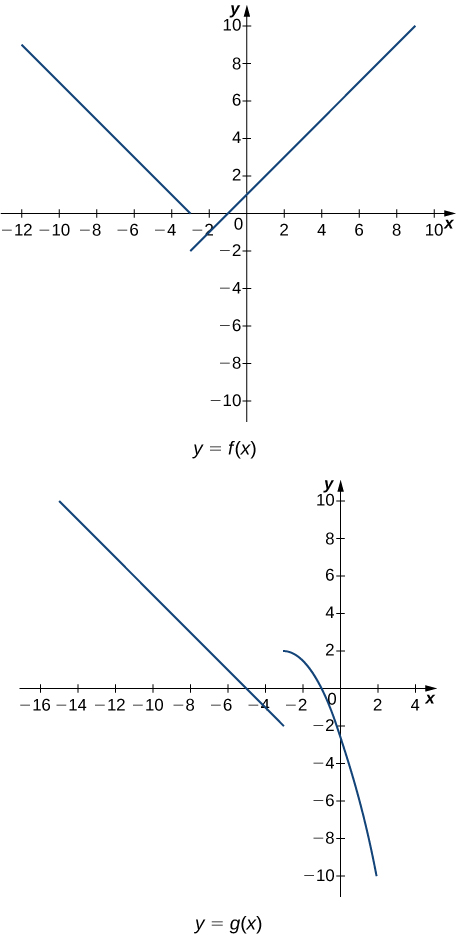
\includegraphics[width=2in]{week03f.jpeg}
\end{center}
\end{prob}

\begin{prob}
\begin{enumerate}[(a)]
\item Use the fact that $(x-2)^2\ge 0$ for all real $x$ to explain why $2x-1\le x^2-2x+3$ for all real $x$.
\item Determine the limits of both $2x-1$ and $x^2-2x+3$ as $x\to 2$.
\item Suppose that $g(x)$ is a function defined on an open interval containing $2$, and suppose that $2x-1\le g(x)\le x^2-2x+3$. Evaluate $\lim_{x\to 2}g(x)$.
\end{enumerate}
\end{prob}

\begin{prob}
\begin{enumerate}[(a)]
\item Let $f(x) = 1-x-x^2$. Use the definition of the derivative and limit laws to determine $f'(0)$.
\item Use your answer from part (a) to determine the equation of the tangent line to $y=f(x)$ at $x=0$.
\item Use desmos or a similar tool to plot $y=f(x)$ and your tangent line to check your solution.
\end{enumerate}
\end{prob}


\end{document}